\documentclass[10pt,a4paper]{article}
\usepackage[utf8]{inputenc}
\usepackage{amsmath}
\usepackage{amsfonts}
\usepackage{amssymb}
\usepackage{natbib}
\usepackage{graphicx}
\usepackage[left=2cm,right=2cm,top=2cm,bottom=2cm]{geometry}
\begin{document}

We discuss a method to filter observed data, $u_\mathrm{obs}$, in a Bayesian framework, where $u_\mathrm{obs}$ can be spatial, temporal, or higher dimensional data.  We are also not limited to cases where $u_\mathrm{obs}$ is observed over a regular grid. Our filtered estimate, $u_\mathrm{post}$, incorporates $u_\mathrm{obs}$ and prior knowledge of the statistical properties of the underlying signal.  In this sense, this work is closely related to Kriging and, more generally, Gaussian process regression \citep[e.g][]{Rasmussen2006} .  We constrain $u_\mathrm{post}$ with the observation equation

\begin{equation}\label{eq:Data}
  u_\mathrm{post} = u_\mathrm{obs} + \epsilon,\ \ \ \epsilon \sim \mathcal{N}(0,\mathbf{C}_\mathrm{obs}),
\end{equation}
and the prior model

\begin{equation}\label{eq:Prior}
  u_\mathrm{prior} \sim \mathcal{N}(0,\mathbf{C}_\mathrm{prior}),
\end{equation}
where $\epsilon$ and $u_\mathrm{prior}$ are considered to be Gaussian processes with zero mean and covariances $\mathbf{C}_\mathrm{obs}$ and $\mathbf{C}_\mathrm{prior}$ respectively.  The solution for $u_\mathrm{post}$ minimizes the objective function  

\begin{equation}\label{eq:Objective}
||u_\mathrm{post} - u_\mathrm{obs}||_{\mathbf{C}_\mathrm{obs}}^2 + 
||u_\mathrm{post}||_{\mathbf{C}_\mathrm{prior}}^2
\end{equation}
and is itself a Gaussian process with a distribution described by

\begin{equation}
  u_\mathrm{post} \sim \mathcal{N}(\bar{u}_\mathrm{post},\mathbf{C}_\mathrm{post}).
\end{equation}
We use $\bar{u}_\mathrm{post}$ and $\mathbf{C}_\mathrm{post}$ to denote the mean and covariance of $u_\mathrm{post}$ respectively.  Using Bayesian linear regression \citep[e.g.][]{Tarantola2005} these values are found to be  

\begin{equation}\label{eq:GeneralSolution}
\begin{split}
  \bar{u}_\mathrm{post} &= (\mathbf{C}_\mathrm{obs}^{-1} + 
                            \mathbf{C}_\mathrm{prior}^{-1})^{-1}
                            \mathbf{C}_\mathrm{obs}^{-1} u_\mathrm{obs}
\\
\mathbf{C}_\mathrm{post} &= (\mathbf{C}_\mathrm{obs}^{-1} + 
                             \mathbf{C}_\mathrm{prior}^{-1})^{-1}.                          
\end{split}
\end{equation}
 
$\mathbf{C}_\mathrm{obs}$ is presumably well known, while $\mathbf{C}_\mathrm{prior}$ needs to be chosen based on an understanding of the underlying signal which we are trying to estimate.  With a judicious choice of $\mathbf{C}_\mathrm{prior}$,  eq. (\ref{eq:GeneralSolution}) can be made equivalent to several well established smoothing methods.  In particular, we demonstrate how eq. (\ref{eq:GeneralSolution}) can be viewed as a low-pass filter with a well defined cutoff frequency. This is first demonstrated for filtering one-dimensional data, and the extension to higher dimensions follows naturally.  

\section*{One-dimensional smoothing}
For one-dimensional data we consider a prior which can be stated implicitly as

\begin{equation}\label{eq:ImplicitPrior1D}
  \mathbf{D}_{n} u_\mathrm{prior} = q, \ \ \ q \sim \mathcal{N}(0,\lambda^2),
\end{equation}  
where $D_n$ is an $n^{th}$ order differentiation matrix, and $q$ is white noise with constant variance $\lambda^2$.  If we momentarily ignore the fact that $D_n$ is not invertible then we can explicitly write our prior covariance as

\begin{equation}\label{eq:ExplicitPrior1D}
\mathbf{C_\mathrm{prior}} = \lambda^2(\mathbf{D}_n^T\mathbf{D}_n)^{-1},
\end{equation}
and the filtered mean and covariance are described by
\begin{equation}\label{eq:1DSolution}
\begin{split}
\bar{u}_\mathrm{post} &= (\mathbf{C}_\mathrm{obs}^{-1} +   
                   \frac{1}{\lambda^2}\mathbf{D}_n^T\mathbf{D}_n)^{-1}\mathbf{C}_\mathrm{obs}^{-1}
                   u_\mathrm{obs}
\\
\mathbf{C}_\mathrm{post} &= (\mathbf{C}_\mathrm{obs}^{-1} +   
                            \frac{1}{\lambda^2}\mathbf{D}_n^T\mathbf{D}_n)^{-1}.
\end{split}
\end{equation}

This filtered solution is closely tied to several well established methods of smoothing.  For example, \citet{Kimeldorf1970} pointed out that eq. (\ref{eq:1DSolution}) is equivalent to a smoothing spline.  This can be seen by ignoring data uncertainty (i.e. $\mathbf{C}_\mathrm{obs}=\mathbf{I}$) and noting from eq. (\ref{eq:Objective}) that $\bar{u}_\mathrm{prior}$ minimizes 

\begin{equation}
||u_\mathrm{obs} - \bar{u}_\mathrm{prior}||_2^2 + ||D_n\bar{u}_\mathrm{prior}||_2^2,
\end{equation}
which is a discretized form of the definition of a smoothing spline \citep[e.g][]{DeBoor1978}.  As another example, we can loosely interpret our prior model in eq. (\ref{eq:ImplicitPrior1D}) as Brownian motion or integrated Brownian motion when $n=1$ and $n=2$, respectively.  From this perspective, it is possible to see the connection between eq. (\ref{eq:1DSolution}) and Kalman filters, where these stochastic models are commonly used to describe time-dependent signals \citep[e.g.][]{Segall1997}.

One challenge that is common to each of these smoothing methods is selecting the hyperparameter $\lambda$.  There are numerous ways that this could be accomplished.  For example, one could use cross-validation, a trade-off curve, or simply vary $\lambda$ until $\bar{u}_\mathrm{post}$ looks appropriate when compared to $u_\mathrm{obs}$.  There is merit to using an entirely objective approach such as cross-validation, and this would be approriate if there is no prior knowledge of the signal's characteristic wavelength.  Otherwise, it may be better to chose $\lambda$ such that eq. (\ref{eq:1DSolution}) damps out all the high frequency oscillations which are known to be noise.  We elaborate on this point by demonstrating that eq. (\ref{eq:1DSolution}) can also be viewed as a low-pass filter with a cutoff frequency determined by $\lambda$.  

We wish to transform $\bar{u}_\mathrm{post}$ in eq. (\ref{eq:1DSolution}) to the frequency domain and in order to do so we assume that $u_\mathrm{obs}$ has a constant sampling rate. We also require that $\epsilon$ and $u_\mathrm{prior}$ are stationary stochastic processes (i.e. their statistical properties are invariant to time shifts).  We require them to be stationary so that matrix multiplication by $\mathbf{C}_\mathrm{obs}$ and $\mathbf{C}_\mathrm{prior}$ can be viewed as convolution in the time domain and thus multiplication in the frequency domain.  We then consider the simplifying case where $\epsilon$ is white noise with constant variance $\sigma^2$ (i.e. $\mathbf{C}_\mathrm{obs} = \sigma^2\mathbf{I}$), and $\mathbf{D}_n$ is the periodic spectral differentiation matrix \citep[e.g.][]{Trefethen2000}.  Under a discrete Fourier transform, $\mathbf{D}_n$ has the properties

\begin{equation}\label{eq:Property1}
  \mathcal{F}[\mathbf{D}_nf] = (2\pi i\omega)^n \hat{f}
\end{equation}
and

\begin{equation}\label{eq:Property2}
  \mathcal{F}[\mathbf{D}^T_nf] = (-2\pi i\omega)^n \hat{f},
\end{equation}
where $\omega$ is the frequency domain variable, $f$ is an arbitrary vector and $\hat{f}$ is its discrete Fourier transform.  The discrete Fourier transform of $\bar{u}_\mathrm{post}$ is then

\begin{equation}\label{eq:1DFourierSoln1}
\hat{u}_\mathrm{post}(\omega) = \frac{\frac{1}{\sigma^2}}
                                  {\frac{1}{\sigma^2} +                  
                                  \frac{(2\pi\omega)^{2n}}{\lambda^2}}
                                  \hat{u}_\mathrm{obs}(\omega).
\end{equation}
We make the change of variables 

\begin{equation}\label{eq:VariableChange}
\lambda^2 = (2\pi\omega_c)^{2N}\sigma^2
\end{equation}
which changes the hyperparameter from $\lambda$ to $\omega_c$.  The reason for this change of variables becomes apparent when we simplify eq. (\ref{eq:1DFourierSoln1}) to

\begin{equation}\label{eq:1DFourierSoln2}
\hat{u}_\mathrm{post}(\omega) = \frac{1}
                                  {1 + \left(\frac{\omega}{\omega_c}\right)^{2n}}
                                  \hat{u}_\mathrm{obs}(\omega).        
\end{equation}
We can recognize eq. (\ref{eq:1DFourierSoln2}) as an n'th order low-pass Butterworth filter with cut-off frequency $\omega_c$.  In the limit as $N\to \infty$ eq. (\ref{eq:1DFourierSoln2}) becomes an ideal low-pass filter which removes all frequencies above $\omega_c$ and leaves lower frequencies unaltered.  Of course, an ideal low-pass filter is often undesirable because it will tend to produce ringing artifacts in the filtered solutions.  When modeling $u_\mathrm{prior}$ as Brownian motion or integrated Brownian motion, where $n=1$ and $n=2$ respectively, the transfer function is tapered across $\omega_c$, which ameliorates ringing in the filtered solution.

By demonstrating that eq. (\ref{eq:1DSolution}) can be made equivalent to a low-pass filter, it may not be clear why we would ever use eq. (\ref{eq:1DSolution}) when it is far more efficient to filter in the frequency domain through the Fast Fourier Transform.  In order to make use of the Fast Fourier Transform, the observations must be made at a constant sampling rate and the observation noise must be  white with constant variance.  In contrast, these conditions do not need to be met in order to evaluate eq. (\ref{eq:1DSolution}).  The question is then whether eq. (\ref{eq:1DSolution}) still effectively acts as a low-pass filter when the idealized conditions are not met.  

We answer this question with a demonstration.  In this demonstration we generate 100 samples of synthetic data over the time interval $0<t<1$ yr.  The true signal in the syntethic data is a sine wave with a frequency of 1 yr$^{-1}$ and 1 mm amplitude.  We obscure the synthetic data with white noise that does not have a constant variance.  We randomly pick a variance for each datum from a uniform random distribution ranging from 0.5 to 2 mm$^2$.  For the period from 1 to 2 years, we assign a variance of 25 mm$^2$ to the data, effectively making the data uniformitive for the filtered solution.  The synthetic data and its estimated power spectral density are plotted in Figure \ref{fig:Demo}.  Our goal is to use eq. (\ref{eq:1DSolution}) as a low-pass filter which damps out frequencies that are higher than our signal.  Since our data does not have constant variance, we cannot choose a cutoff frequency from eq. (\ref{eq:VariableChange}).  Instead we define a characteristic data variance as
\begin{equation}
\frac{1}{\bar{\sigma^2}} = \frac{1}{P} \mathrm{tr}\left(\mathbf{C}_\mathrm{obs}^{-1}\right),
\end{equation}
where $P$ is the number of observations, and we relate $\lambda$ to $\omega_c$ by
\begin{equation}
\lambda^2 = (2\pi\omega_c)^{2n}\bar{\sigma}^2.  
\end{equation}
In this demonstration $D_n$ is still the spectral differentiation matrix and we use $n=2$. Our cutoff frequency is chosen to be $\omega_c=2$ yr$^{-1}$.  The filtered solution and its frequency content are plotted Figure \ref{fig:Demo}, where it is apparent that eq. (\ref{eq:1DSolution}) is indeed acting as a low-pass filter with the specified cut-off frequency even though the variances are not constant. It is worth noting that the frequency content of $u_\mathrm{post}$ appears to change depending on the variance of $u_\mathrm{obs}$. For example, Over the interval $1<t<2$, where the variance of $u_\mathrm{obs}$ is higher, $u_\mathrm{post}$ lacks the higher frequency oscillations that can be seen in the remainder of the time series. This is desirable behavior because we do not want $u_\mathrm{post}$ contorting to fit dubious data.  It is also worth pointing out that $u_\mathrm{post}$ asymptotically approaches a solution that is not significantly different from that shown in Figure \ref{fig:Demo} when the variance for $u_\mathrm{obs}$ increases to infinity over the interval $1<t<2$.  This too is desirable behaviour because one could then surmise that an appropriate way to handle missing data with eq. (\ref{eq:1DSolution}) is to assign $u_\mathrm{obs}$ an infinite variance for the missing time period.  With this insight, we can then extend the application of eq. (\ref{eq:1DSolution}) from data smoothing to data interpolation and extrapolation.   

\begin{figure}
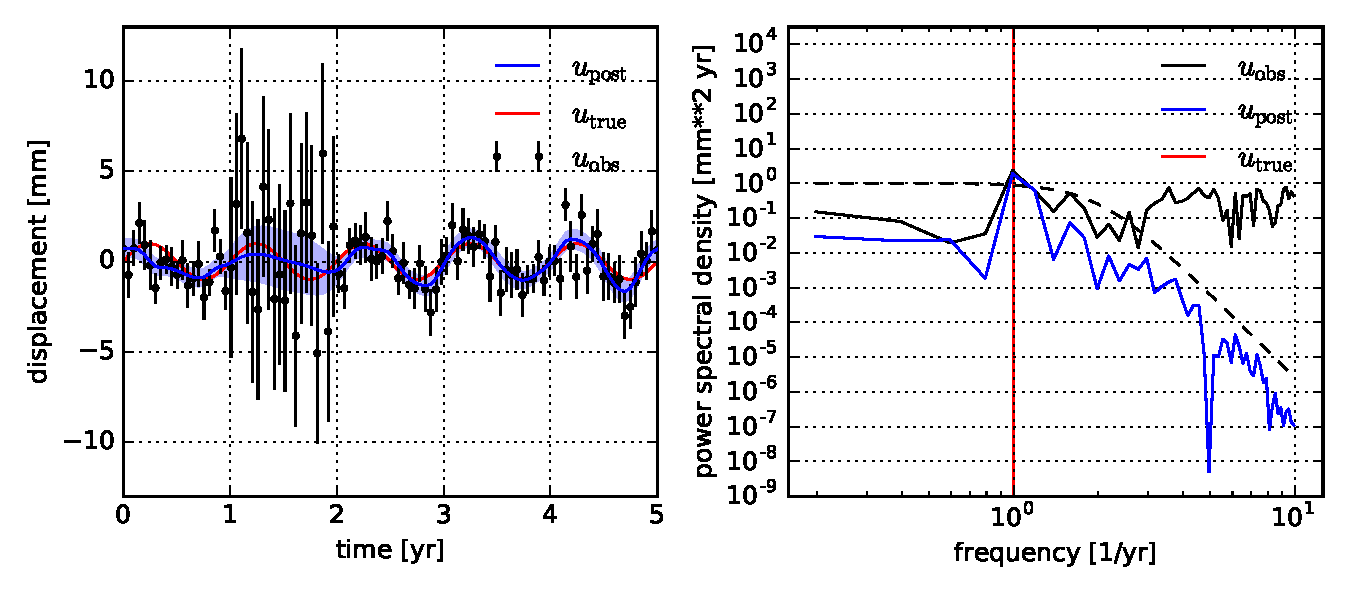
\includegraphics[scale=0.75]{figures/fig1}
\caption{Left panel shows observed data (black scatter points), filtered data (blue line), and the true signal which we are trying to recover (red line).  The lines on each scatter point and the light blue region show the one standard deviation uncertainty for the observations and filtered solution respectively.  The right panel shows the estimated power spectral density for the observed, filtered, and true signal.  The black dashed line is the squared transfer function in eq. (\ref{eq:1DFourierSoln2}) with $\omega_c=2$ yr$^{-1}$, which roughly indicates how eq. (\ref{eq:1DSolution}) scales the frequency content of $u_\mathrm{obs}$.  If the data variances were constant then the frequency content of $u_\mathrm{obs}$ and $u_\mathrm{post}$ would be exactly related by the black dashed line.}   
\label{fig:Demo}
\end{figure}

\section*{Smoothing in higher dimensions} 
We expand our discussion from one-dimensional smoothing to smoothing in two-dimensional space.  While the remainder of this paper discusses smoothing in two-dimensions, the extension to smoothing in higher dimensions will prove to be trivial.  We now allow $u_\mathrm{prior}$ to have non-zero covariance along multiple dimensions.  In other words, we now treat $u_\mathrm{prior}$ as a random field rather than a stochastic process.  The smoothed solution that we seek is still given by eq. \ref{eq:GeneralSolution} and our task is once again to find an appropriate choice of $\mathbf{C}_\mathrm{prior}$.  Below we consider the case where the $M$'th order Laplacian of $u_\mathrm{prior}$ is white noise.  That is to say
\begin{equation}
  \mathbf{\Delta}_M u_\mathrm{prior}(x_1,x_2) = q, \ \ \ q \sim \mathcal{N}(0,\lambda^2)
\end{equation}  
where 
\begin{equation}\label{Laplacian}
\mathbf{\Delta}_M = \frac{\partial^{2M}}{\partial x_1^{2M}} +
           \frac{\partial^{2M}}{\partial x_2^{2M}}.
\end{equation} 
The corresponding covariance matrix is then
\begin{equation}\label{Covariance2D}
\mathbf{C}_\mathrm{prior} = \lambda^2\left(\mathbf{\Delta}_M^T\mathbf{\Delta}_M\right)^{-1}. 
\end{equation}           
We again assume that the observation noise is uncorrelated with constant variance $\sigma^2$.  Using the change of variables
\begin{equation}
\lambda = (2\pi\omega_c)^{2M}\sigma
\end{equation}
we obtain the solution
\begin{equation}\label{eq:TimeSoln2d}
u_\mathrm{smooth}(x_1,x_2) = \left(\mathbf{I} + 
                          \left(\frac{1}{2\pi\omega_c}\right)^{4M}
                          \mathbf{\Delta}_M^T\mathbf{\Delta}_M\right)^{-1}
                          u_\mathrm{obs}(x_1,x_2),
\end{equation}
which in the two-dimensional frequency domain is
\begin{equation}\label{eq:FourierSoln2d}
\hat{u}_\mathrm{smooth}(\omega_1,\omega_2) = \frac{1}{1 + \left(\frac{\omega_1^{2M} + \omega_2^{2M}}
                                                  {\omega_c^{2M}}\right)^2}
                                             \hat{u}_\mathrm{obs}(\omega_1,\omega_2).
\end{equation}
The transfer function in eq. (\ref{eq:FourierSoln2d}) can once again be recognized as a low-pass filter.  Namely, in the limit as $M \to \infty$ all the frequency pairs, $(\omega_1,\omega_2)$, where $|\omega_1| > \omega_c$ or $|\omega_2| > \omega_c$ are removed.  That is, the transfer function becomes a two-dimensional box centered at $(0,0)$ with width $2\omega_c$.  It is apparent from the transfer function why our prior model must be defined in terms of even order derivatives.  If eq. (\ref{Laplacian}) contained odd order derivatives, then all frequency pairs where $\omega_1=-\omega_2$ would be unattenuated, leaving undesirable artifacts in the smoothed solution.

We have demonstrated with eq. (\ref{eq:TimeSoln} and \ref{eq:TimeSoln2d}) that eq. \ref{eq:GeneralSolution} can effectively act as a low pass filter with a judicious choice of $\mathbf{C}_\mathrm{prior}$.  One may then wonder why eq. (\ref{eq:TimeSoln} and \ref{eq:TimeSoln2d}) would ever be used to smooth data when it is far more efficient to perform the equivalent operation through the Fast Fourier Transform domain.  The power in eq. (\ref{eq:TimeSoln} and \ref{eq:TimeSoln2d}) resides in the fact that they makes no assumption about when or where the observations have been made.  In order to filter data through the Fast Fourier Transform, the observations must be evenly spaced on a regular grid, which is often not the case for geophysical data.  Indeed,  the focus of this paper is to smooth data which has been observed at scattered locations.  We can use eq. (\ref{eq:TimeSoln} and \ref{eq:TimeSoln2d}) regardless of where the observations were made provided that we are able to create the differentiation matrix.  We use the recently developed Radial Basis Function Finite-Difference method to form the differentiation matrices and we describe the procedure in the follow section. 

\bibliographystyle{apalike}
\bibliography{mybib}  

 
\end{document}